Jane's use case involves groups and actions, polynomials, rings and ideals, and Gröbner bases, all of which must be formalized in the MitM ontology.
Due to space restrictions, we only describe the ontology for computational group theory (CGT) as an example.
This formalization can be found at~\cite{mitm:groups:on}.
% \ednote{FR@all: This section is incomplete -  it lacks the description rings etc. This must be fixed but cannot be fixed on short notice. So I'm carefully phrasing this paragraph to work around it.}

\subsection{Foundation}

\OMMT formalizations must be relative to foundational logic, which is itself formalized in \OMMT.
As foundation for all formalizations in MitM \cite{mitm:foundation:on}, we use a polymorphic dependently typed $\lambda$-calculus with two universes \lstinline|type| and \lstinline|kind| (roughly analogous to sets and proper classes in set theory) and subtyping.
It provides dependent function types \lstinline|{a:A}B(a)|, representing the type of all functions mapping an argument \lstinline|a:A| to some element of type \lstinline|B(a)|. If \lstinline|B| does not depend on the argument \lstinline|a|, we obtain the simple function type \lstinline[mathescape]|A$\to$B|.

For formulas, we use a type \lstinline|prop| and a higher order logic where quantifiers range over any type.
We furthermore follow the judgments-as-type paradigm by declaring a function \lstinline[mathescape]|$\vdash$:prop$\to$type| mapping propositions to the \defemph{type of their proofs}, which allows us to declare proof rules as functions mapping proofs (of the premises) to a proof (of the conclusion).

The judgment \lstinline|A<:B| expresses that $A$ is a subtype of $B$.
We use power types (the type of subtypes of a type) and predicate subtyping \lstinline?{'a:A | P(a)'}?.
The latter makes type-checking undecidable, but that is necessary for natural formalizations in many areas of mathematics.

\begin{figure}[ht]\centering
  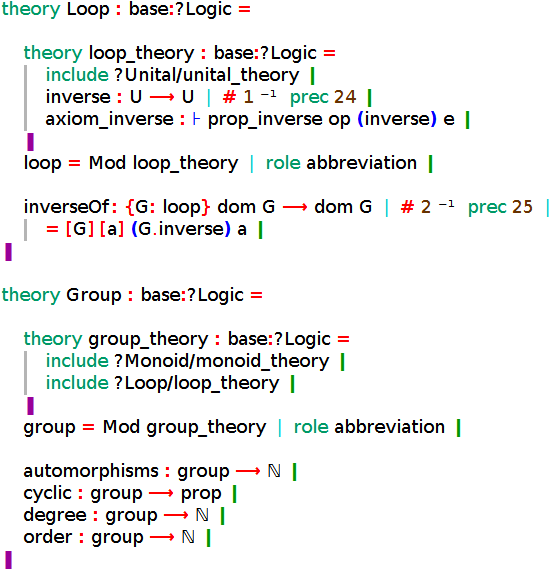
\includegraphics[width=8cm]{../D6.8/groups}
  \caption{MitM Ontology Fragment}\label{fig:mitm1}
\end{figure}

A critical question is what additional types to provide.
To be practical at all, this must include basic types for aggregation (e.g., records) and collection (e.g., lists).
Based on a survey of practical needs, we compiled such a set in Deliverable \textbf{D6.8.}~\cite{ODK-D6.8,}

Moreover, we need an open-ended set of types for mathematical structures such as fields and rings.
Here we have developed a novel type constructor~\cite{MueRabKoh:tat18} that turns any MMT theory into the corresponding dependent record type.
This combines the benefits of MMT's axiomatic theories and a flexible type system.
Concretely, for a theory \lstinline|T|, the type \lstinline|Mod T| is the record type of models of \lstinline|T|.
For example, in Figure~\ref{fig:mitm1} we define groups in terms of an MMT theory \lstinline|group_theory| that declares the operations and axioms in a way that corresponds to the mathematical definition of groups.
Then \lstinline|group=Mod group_theory| is the type of all models of that theory, i.e., the type of groups.
Any element \lstinline|g:group| thus represents an actual group, whose operations and axioms can be accessed via record field projections (e.g. \lstinline|g.inverse| yields the inverse operation of \lstinline|g| (imported from loops via the \lstinline|include ?Loop/loop_theory|-statement).
Since axioms are turned into record type fields as well, actually constructing a record of type \lstinline|group| corresponds to proving that the field \lstinline|universe| and the operations provided in the record do in fact form a group.

\subsection{Domain Ontologies}

Relative to the foundation, we can formalize the actual mathematical knowledge we are interested in.
As a running example, we describe a formalization of computational group theory (CGT), which is inspired by the corresponding implementation in \GAP.
It uses several different levels of abstraction -- currently \emph{abstract}, \emph{representation}, \emph{implementation}, and \emph{concrete}.
From our experience, we expect this pattern to be applicable across computational algebra, possibly with additional levels of abstraction. 
The left box in Figure \ref{fig:cgtontology} shows the levels and their relation to the constructors and operations of \GAP.

\begin{figure}[ht]\centering
  \tikzinput[width=.98\textwidth]{alignmentimg}
  \caption{Alignments between the MitM Ontology and the \GAP API}\label{fig:cgtontology}
\end{figure}

\paragraph{Abstract Level} This contains the theory of \emph{Groups}: the group
axioms, generating sets, homomorphisms, group actions, stabilisers, and orbits.
This also easily leads into definitions of centralisers -- i.e. stabilisers of
elements under conjugation -- and normalisers -- i.e. stabilisers of subgroups
under conjugation, stabiliser chains, Sylow-$p$ subgroups, Hall subroups, and
many other concepts.

\OMMT also allows expressing that there are different equivalent definitions of
a concept: We defined group actions in two ways and used \emph{views} to express
their equivalence.

\paragraph{Representation Level} 
Abstract groups are represented in different ways as concrete objects
suitable for computation: as groups of permutations, groups of matrices,
finitely presented groups, algebraic constructions of groups, or using
polycyclic presentations.

%Additionally, mathematicians often compute with canonical representatives of an
%isomorphism class of groups: When group theorists talk about the ``Dihedral
%group of order 8'', they often have a particular representation in mind, for
%example as a group that acts on the square by rotations and reflections. In \GAP
%this group would be represented as a group of permutations, or by a polycyclic
%presentation.

Many representations arise naturally from \emph{group actions}: If we are
considering symmetry in a setting where we want to apply group theory, we start
with a group action, for example a group acting on a graph by permuting its
vertices.

% \ednote{MP@ALL: More concrete? More ``gripping''? I already
% talked about the canonical example with the dihedral group}

The universal tool to bridge the gap between groups, representations and
canonical representatives are \emph{group homomorphisms}, particularly
embeddings and isomorphisms, which are used extensively in \GAP. This is
reflected in our approach.

\paragraph{Implementation Level}
At this level we encode implementation details: Permutation groups in \GAP
are considered as finite subgroups of the group $S_{\mathbb{N}+}$, and defined by
providing a set of generating permutations. \GAP then computes a stabiliser chain
for a group that was defined this way, and naturally considers the group to be a
subgroup of $S_{[1..n]}$, where $n$ is the largest point moved.

\paragraph{Concrete Level}
It is at the concrete level where the computation happens: while the higher levels
are suitable for mathematical deduction and inference, this level is where \GAP
(or any other system providing computational group theory) does its work.
If a group (or a group action) has been constructed by giving generators
through MitM, \GAP can now compute the size of the group, its isomorphism type,
and perform all the other operations that are available via the \GAP system
dialect.

%\begin{oldpart}{MK: This was commented out in the MACIS paper; maybe we can use this somewhere?}
%For example, if one creates \lstinline|Group((1,2,3,4,5,6,7,8,9,10,11),(3,7,11,8)(4,10,5,6))|
%in \GAP, then one can compute the size of this group, which is $7920$, determine
%whether it is abelian (which it is not), or compute its Sylow-$2$ subgroups.
%
%Coming back to the usefulness of isomorphisms, creating the group
%\begin{lstlisting}
%Group((1,5,7)(2,9,4)(3,8,10), (2,6)(3,5)(4,7)(9,10), (1,11)(2,7)(3,5)(4,6),
%(2,5)(3,6)(4,7)(11,12))
%\end{lstlisting}
%we can find an isomorphism between these two groups, and knowing the Sylow-$2$
%subgroups of the first one can deduce the Sylow-$2$ subgroups of the second one.
%
%There are other ``canonical'' representatives of this group; there are $5040$ conjugates
%of $M_{11}$ inside the symmetric group on $11$ points alone, and the \GAP primitive groups
%library contains $5$ representations of $M_{11}$, as subgroups of the symmetric group on
%$11$, $12$, $55$, $66$, and $165$ points.
%
%While the groups are isomorphic, hence we could construct isomorphisms between
%them, their action on the points are not .
%
%Here it becomes clear how the layers of abstraction work as a means of picking the correct
%translation:
%
%\paragraph{Evaluation}
%Building this part of the CGT MitM Ontology already posed a few challenges for the \MMT
%system, mostly to do with subtyping, since we needed to be able to talk about all
%subgroups of a group, and all normal subgroups of a group. Quantifying over these classes
%can lead to inconsistencies in the underlying type theory.  These challenges immediately
%translate into necessary features in \OMMT, for example by introducing universe
%hierarchies.  \ednote{MP@FR+DM: I commented this out because I believe the paragraph above
%  describes what was done in MMT to accommodate for the CGT MitM ontology}
%\end{oldpart}

\ednote{FR: the formalization of elliptic curves could be moved here as a second example}

%%% Local Variables:
%%% mode: latex
%%% TeX-master: "report"
%%% End:

%  LocalWords:  sec:cgt MueRoYuRa:abtafs17,MueGauKal:cacfms17 emph Sylow subroups medskip formalizations mcpoot13 wrapfigure vspace
%  LocalWords:  mathbb fig:cgtontology alignmentimg smallskip subtyping organization
%  LocalWords:  centering tikzinput textwidth rotercentations lstinline lstinline vdash
%  LocalWords:  type:kind mathescape conclusio fig:mitm1 g:group includegraphics mitm1
%  LocalWords:  lstlisting Gröbner formalized formalizing formalization ednote defemph
%  LocalWords:  textbf MueRabKoh:tat18 oldpart
